\chapter{Proposed algorithm}
\label{cha:proposed_algorithm} % (fold)
Our approach only uses a latent basis over the policy space instead of using one over the policy space and another one over the descriptor space like in \cite{Isele2016UsingLearning}.\\
Again, for a task $(t)$, we can reconstruct the policy using the shared basis $L$ and the sparse coefficients over this basis for that specific task $s^{(t)}$: $\theta^{(t)} = Ls^{(t)}$, with $\theta^{(t)} \in \mathbb{R}^d$, $L \in \mathbb{R}^{d \times k}$ and $s^{(t)} \in \mathbb{R}^k$.\\
The architecture of the network used for one task is visualized in Figure~\ref{fig:algonn}.
\begin{figure}[htb]
    \centering
    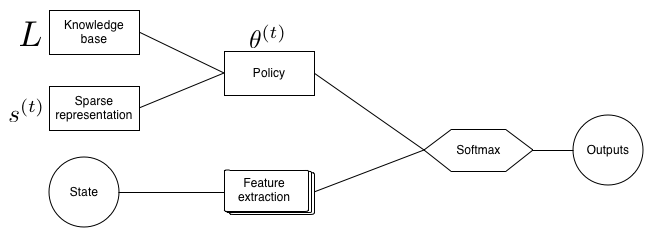
\includegraphics[width=\linewidth]{images/knowledge_transfer.png}
    \caption[Artificial neural network architecture used in our approach]{Artificial neural network architecture used in our approach. The sparse representation $\theta^{(t)}$ is different for every task $(t)$, while the same knowledge base is used for every task.}
    \label{fig:algonn}
\end{figure}

The source tasks can be learned in two ways. They can be learned either sequentially or in parallel.
In the sequential way, we collect trajectories and calculate the gradients for every task after another. These gradients include both those for the sparse representation and for the knowledge base. They are calculated for every episode of a task like in the \texttt{REINFORCE} algorithm (explained in Section~\ref{sub:rl_policy_gradient}), i.e. with likelihood ratios using discounted rewards as a sample for the $Q$ values of the policy.\\
After evaluating every task, we sum and apply all of their gradients. The learning process for the source tasks then stops when a certain number of updates have been applied.\\
In the parallel way, all source tasks are learned at the same time, each executing a certain number of updates. Trajectories are collected for each task continuously and its gradients are applied immediately after they are calculated. This means that they are not first summed up like in the sequential method.\\
The resulting pseudo code for the source tasks learned using the parallel method can be seen in Algorithm~\ref{algo:ownsource}.\\
\begin{algorithm}[htb]
\DontPrintSemicolon
\emph{// Assume global knowledge base $L$ and global shared counter $T \gets 0$}\;
% \emph{// Assume thread-specific parameter vector $\theta_g'$}\;
Initialize thread-specific parameter vector $\theta^{(t)}$\;
Initialize thread step counter $t\gets 1$\;
\Repeat{$T > T_{max}$}{
    $\theta^{(t)} \gets Ls^{(t)}$\;
    Reset gradients: $d\theta^{(t)} \gets 0$\;
    % Synchronize agent-specific parameters  $\theta_g' \gets \theta_g$\;
    $t_{start} \gets t$\;
    Initialize state $s_t$\;
    \Repeat{terminal $s_t$ \textbf{or} $t-t_{start} = t_{max}$}{
        Perform $a_t$ according to policy $\pi(a_t \vert s_t;\theta^{(t)})$\;
        Receive reward $r_t$ and new state $s_{t+1}$\;
        $t \gets t + 1$\;
        $T \gets T + 1$\;
        }
    \For {$i \in \{t-1,\dots,t_{start} \}$} {
        %Accumulate gradients w.r.t. $\theta'$: $d\theta \gets d\theta + \nabla_{\theta'} \log\pi(a_i|s_i;\theta') (R - V(s_i;\theta'_v))$\;
        Accumulate gradients w.r.t. $\theta^{(t)}$: $\theta^{(t)} \gets \theta ^{(t)}+ \alpha \nabla_{\theta^{(t)}} \log \pi_{\theta^{(t)}}(s_t,a_t)v_t$\;
    }
    Perform asynchronous update of $\theta^{(t)}$ using $d\theta^{(t)}$\;
}
\caption[Asynchronous knowledge transfer agent for a source task]{Asynchronous knowledge transfer agent for a source task.}
\label{algo:ownsource}
\end{algorithm}

After learning the source tasks, the knowledge base that they jointly learned is transferred to the target task. This task then separately learns and executes updates for a number of episodes. The pseudo-code for the target task is shown in Algorithm~\ref{algo:owntarget}.\\
\begin{algorithm}[htb]
\DontPrintSemicolon
\emph{// Assume global knowledge base $L$}\;
Initialize task-specific sparse representation $s^{(t)}$\;
Initialize thread step counter $t\gets 1$\;
\Repeat{$T > T_{max}$}{
    $t_{start} \gets t$\;
    Initialize state $s_t$\;
    \Repeat{terminal $s_t$ \textbf{or} $t-t_{start} = t_{max}$}{
        Perform $a_t$ according to policy $\pi(a_t|s_t;L  s^{(t)})$\;
        Receive reward $r_t$ and new state $s_{t+1}$\;
        $t \gets t + 1$\;
        }
    \For {$i \in \{t-1,\dots,t_{start} \}$} {
        %Accumulate gradients w.r.t. $\theta'$: $d\theta \gets d\theta + \nabla_{\theta'} \log\pi(a_i|s_i;\theta') (R - V(s_i;\theta'_v))$\;
        Accumulate gradients w.r.t. $s^{(t)}$: $s^{(t)} \gets s^{(t)} + \alpha \nabla_{s^{(t)}} \log \pi_{s^{(t)}}(s_t,a_t)v_t$\;
    }
    Perform update of $s^{(t)}$ using $ds^{(t)}$\;
}
\caption[Knowledge transfer agent for the target task]{Knowledge transfer agent for the target task.}
\label{algo:owntarget}
\end{algorithm}
% section proposed_algorithm (end)
